% --------------------------------------------------------------------------
% Report template for BIR projects
% Report template with support for Portuguese and English languages
% Change language {brazil or english} in \documentclass as per the examples
% This template has support for the ABNT citing format
% 
% Original version: jan/2019
% https://github.com/
% 
% Based on ABNTEX2 and the thesis template
% --------------------------------------------------------------------------
\documentclass[
%\DeclareUnicodeCharacter{200B}{}
% --------------------------------------------------------------------------
% classe memoir . options                                                   
12pt,					% tamanho da fonte
openright,				% cap. começam em pág ímpar (ins pág vazia caso preciso)
oneside,				% para impressão em verso e anverso. Oposto a oneside
a4paper,				% tamanho do papel
% --------------------------------------------------------------------------
% classe abntex2 . options                                                  
%chapter=TITLE,			% títulos de capítulos convertidos em letras maiúsc.
%section=TITLE,			% títulos de seções convertidos em letras maiúsc.
%subsection=TITLE,		% títulos de subseções convertidos em letras maiúsc.
%subsubsection=TITLE,	% títulos de subsubseções convertidos em letras maiúsc.
% --------------------------------------------------------------------------
% Opções de IDIOMA do pacote babel                                          
english,
brazil
]{ABNT/abntex2_report}
% --------------------------------------------------------------------------
% Pacotes básicos    
\usepackage{lmodern}			% Usa a fonte Latin Modern			
\usepackage[T1]{fontenc}		% Selecao de codigos de fonte.
\usepackage[utf8]{inputenc}		% Codificacao do documento (conversão automática dos acentos)
\usepackage{indentfirst}		% Indenta o primeiro parágrafo de cada seção.
\usepackage{color}				% Controle das cores
%\usepackage{graphicx}			% Inclusão de gráficos
\usepackage{microtype} 			% para melhorias de justificação
\usepackage{lipsum}	
\usepackage[brazilian,hyperpageref]{backref} % páginas com citações na bibliog.
%\usepackage[alf,abnt-etal-list=0,abnt-etal-cite=3,abnt-emphasize=bf]{abntex2cite}
\usepackage[alf]{abntex2cite}
%	
\usepackage{lastpage}			% Usado pela Ficha catalográfica
%\usepackage{subfig}
\usepackage{supertabular}       % tabela na capa do documento
\usepackage{booktabs}
\usepackage[table,xcdraw]{xcolor}
\usepackage{adjustbox}
\usepackage{amssymb,amsmath,mathrsfs}
\usepackage{algorithm,algpseudocode}
\usepackage{pgfplots}
\usepackage{tikz}
\usepackage{titlesec}
\usepackage{ragged2e}
\usepackage{tocloft}
\usepackage{threeparttable}
\usepackage{etoolbox}
\usepackage[normalem]{ulem}
\usepackage{yaacro}
\usepackage[none]{verlab}
%\usepackage{fontspec}
%\setmainfont{Helvetica Light}
\usepackage{lscape}
% \usepackage[graphicx]{realboxes}
\usepackage{rotating}
\usepackage{wrapfig}
\usepackage{caption}
\usepackage{subcaption}
\usepackage{dirtytalk}
\usepackage{pdfpages}
\usepackage{threeparttable}
\usepackage{hyperref}
%\hypersetup{draft}
\usepackage{lettrine}
\usepackage{float}
\usepackage{lscape}
\usepackage{adjustbox}
%R - LATEX
\makeatletter
\def\maxwidth{ %
  \ifdim\Gin@nat@width>\linewidth
    \linewidth
  \else
    \Gin@nat@width
  \fi
}
\makeatother

\definecolor{fgcolor}{rgb}{0.345, 0.345, 0.345}
\newcommand{\hlnum}[1]{\textcolor[rgb]{0.686,0.059,0.569}{#1}}%
\newcommand{\hlstr}[1]{\textcolor[rgb]{0.192,0.494,0.8}{#1}}%
\newcommand{\hlcom}[1]{\textcolor[rgb]{0.678,0.584,0.686}{\textit{#1}}}%
\newcommand{\hlopt}[1]{\textcolor[rgb]{0,0,0}{#1}}%
\newcommand{\hlstd}[1]{\textcolor[rgb]{0.345,0.345,0.345}{#1}}%
\newcommand{\hlkwa}[1]{\textcolor[rgb]{0.161,0.373,0.58}{\textbf{#1}}}%
\newcommand{\hlkwb}[1]{\textcolor[rgb]{0.69,0.353,0.396}{#1}}%
\newcommand{\hlkwc}[1]{\textcolor[rgb]{0.333,0.667,0.333}{#1}}%
\newcommand{\hlkwd}[1]{\textcolor[rgb]{0.737,0.353,0.396}{\textbf{#1}}}%
\let\hlipl\hlkwb

\usepackage{framed}
\makeatletter
\newenvironment{kframe}{%
 \def\at@end@of@kframe{}%
 \ifinner\ifhmode%
  \def\at@end@of@kframe{\end{minipage}}%
  \begin{minipage}{\columnwidth}%
 \fi\fi%
 \def\FrameCommand##1{\hskip\@totalleftmargin \hskip-\fboxsep
 \colorbox{shadecolor}{##1}\hskip-\fboxsep
     % There is no \\@totalrightmargin, so:
     \hskip-\linewidth \hskip-\@totalleftmargin \hskip\columnwidth}%
 \MakeFramed {\advance\hsize-\width
   \@totalleftmargin\z@ \linewidth\hsize
   \@setminipage}}%
 {\par\unskip\endMakeFramed%
 \at@end@of@kframe}
\makeatother

\definecolor{shadecolor}{rgb}{.97, .97, .97}
\definecolor{messagecolor}{rgb}{0, 0, 0}
\definecolor{warningcolor}{rgb}{1, 0, 1}
\definecolor{errorcolor}{rgb}{1, 0, 0}
\newenvironment{knitrout}{}{} % an empty environment to be redefined in TeX
\usepackage{alltt}
\IfFileExists{upquote.sty}{\usepackage{upquote}}{}
\DeclareUnicodeCharacter{200B}{}
% --------------------------------------------------------------------------%
% Configurações do PDF final                                                
\definecolor{blue}{RGB}{41,5,195}
\makeatletter
\hypersetup{
	%pagebackref=true,
	pdftitle={\@title}, 
	pdfauthor={\@author},
	pdfsubject={\@title},
	%pdfsubject={\imprimirpreambulo},
	pdfcreator={LaTeX with abnTeX2},
	pdfkeywords={abnt}{latex}{abntex}{abntex2}{\imprimirpalavraschave}, 
	colorlinks=true,       		% false: boxed links; true: colored links
	linkcolor=blue,          	% color of internal links
	citecolor=blue,        		% color of links to bibliography
	filecolor=magenta,      	% color of file links
	urlcolor=blue,
	bookmarksdepth=4
}
%\makeatother
% --------------------------------------------------------------------------
% Posiciona figuras e tabelas no topo da página quando adicionadas sozinhas
% em um página em branco. Ver https://github.com/abntex/abntex2/issues/170
%\makeatletter
\setlength{\@fptop}{5pt} % Set distance from top of page to first float
\makeatother
% --------------------------------------------------------------------------
% Formatação                                                                
\newcommand\tab[1][1cm]{\hspace*{#1}}
\apptocmd{\thebibliography}{\justifying}{}{} 
\renewcommand{\ABNTEXsectionfont}{\bfseries}
\titlespacing*{\chapter}{0pt}{0pt}{12pt}
\titlespacing*{\section}{0pt}{6pt}{6pt}
\titlespacing*{\subsection}{0pt}{6pt}{6pt}
\titlespacing*{\subsubsection}{0pt}{6pt}{6pt}
% --------------------------------------------------------------------------
% Rearranja os finais de cada estrutura                                     
\algrenewtext{EndWhile}{\algorithmicend\ \algorithmicwhile}
\algrenewtext{EndFor}{\algorithmicend\ \algorithmicfor}
\algrenewtext{EndIf}{\algorithmicend\ \algorithmicif}
\algrenewtext{EndFunction}{\algorithmicend\ \algorithmicfunction}
% --------------------------------------------------------------------------
% Espaçamentos entre linhas e parágrafos                                    
\setlength{\parindent}{1.3cm} % linha
\setlength{\parskip}{0.2cm} % parágrafo, tente também \onelineskip
% --------------------------------------------------------------------------
% Informações de dados para CAPA e FOLHA DE ROSTO                           
% \prodtecnica{001 / 2020}
\titulo{Avaliação do Sistema de Medição - TIMON 2.5}
% \tiporelatorio{Parcial} 
% \nomeprojeto{Conceitual - UGV-C}
\outrossubtitulos{~} % opcional
\autores{
	Jéssica Lima Motta\\
	Leonardo Mendes de Souza Lima\\
	Miguel Felipe Nery Vieira\\
	Vinícius José Gomes de Araujo Felismino\
	
}
% \newcommand{\autoresexternos}{
% 	Marco Antonio dos Reis\\
% 	Rebeca Tourinho Lima\
% }
\local{Salvador\\Bahia, Brasil}
\data{Julho de 2020}
% \classificacao{( ) Confidencial  (X) Restrito  ( )  Uso Interno  ( ) Público}
% \revisao{01}
% \tabelacutter{000} 
% \palavraschave{1.Mobile Robots . 2. Disinfection. 3. Autonomous.}
% \classificacaoassunto{000} % Número de Classificação do assunto 
%\parceirologo{logos/x.png}
%------------------------------------------------------------------
% Finalização das configurações da capa
%
%
%------------------------------------------------------------------              
% Acrônimos :: Chamar no texto como \ac{DoF}                                
\begin{acgroupdef}[list=acronyms]
	% \acdef{AHP}{Analytic Hierarchy Process}
	% \acdef{CPU}{Central Process Unit}
	% \acdef{FPS}{Frames Per Second}
	% \acdef{GPS}{Glopal Positioning System}
	% \acdef{IDE}{Integrated Development Environment}
	% \acdef{IMU}{Initial Measurement Unit}
	% \acdef{INS}{Inertial Navigation System}
	% \acdef{LCD}{Liquid Crystal Display}
	% \acdef{LED}{Light-emitting Diode}
	% \acdef{LIDAR}{Light Detection and Ranging}
	% \acdef{PTZ}{Pan-Tilt-Zoom}
	% \acdef{PWM}{Pulse Width Modulation}
	% \acdef{QFD}{Quality Function Deployment}
	% \acdef{ROS}{Robot Operating System}
	% \acdef{RoSA}{Robótica e Sistemas Autônomos}
	% \acdef{SLAM}{Simultaneous Localization and mapping}
	% \acdef{SOTA}{Study of the State of the Art}
	% \acdef{UART}{Universal Asynchrounous Receiver/Transmiter}
	% \acdef{UGV}{Unmanned Ground Vehicle}
	% \acdef{UV}{Ultravioleta}

	% \acdef{DoF}{Degrees of Freedom}
	% \acdef{PoC}{Proof of Concept, em português Prova de Conceito}
	% \acdef{UUV}{Unmanned Underwater Vehicle, em português Veículo Subaquático Não-tripulado}
	% \acdef{AUV}{Autonomous Underwater Vehicle, em português Veículo Subaquático Autônomo}
	% \acdef{UVM}{Unmanned Vehicle Morphing}
	% \acdef{SLAM}{Simultaneous Localization and Mapping}
	% \acdef{ROV}{Remotely Operated Vehicle}
	% \acdef{SOTA}{Study Of The Art}
	% %
	%
	%
\end{acgroupdef}
% --------------------------------------------------------------------------
% Criação do sumário
% \makeindex
%
\begin{document}
	\begin{center}
		\begin{figure}[htp]
			\centering
			\ifelsenotempty{\imprimirparceirologo}{
				\raisebox{-0.5\height}{\includegraphics[height=1.2cm]{\imprimirparceirologo}}
				\hspace{\fill}
				\raisebox{-0.5\height}{
\includegraphics[height=1.2cm]{logos/LogoFiebSenai.png}}
			}{
				\hspace{\fill}
				\raisebox{-0.5\height}{
\includegraphics[height=1.2cm]{logos/LogoFiebSenai.png}}
			}
		\end{figure}
	\end{center}

	% \frenchspacing
	% \imprimircapa
	\MakeUppercase{\textbf{\imprimirtitulo}}\\
	\centering\small{\mainsubsubtitle}\\
	\begin{flushright}
		\imprimirautores		
	\end{flushright}
	% \imprimircatalografica
% --------------------------------------------------------------------------
% Sumário executivo                                                         
% 	\ABNTEXchapterfont\large\textbf{\execsummarytitlename}
% 	\begin{flushleft}
% 		\normalsize
% 		\justify
% 		\normalfont
% 		O projeto UGV-C, também conhecido como \textbf{CAPIVARA} se configura sob o Programa de Formação de Jovens Talentos do Laboratório de Robótica e Sistemas Autônomos do Senai Cimatec. Diante da forte demanda para implementação de soluções contra o virús chinês (COVID-19)em nossa sociedade, o Senai Cimatec firmou compromisso financeiro e humano para o desenvolvimento de plataformas robóticas utilizando em sua grande maioria componentes nacionalizados e de localização no Brasil, sendo assim o Senai Cimatec é o principal fomentador do projeto. O \textit{kick-off} do projeto foi no dia 15/06/2020. O prazo de execução foi planejado para 90 dias.
% 	\end{flushleft}
% 	\clearpage
% %------------------------------------------------------------------
% % Resumo e abstract                                                         
% 	\ABNTEXchapterfont\large\textbf{\resumoatitlename}
% 	\begin{flushleft}
% 		\normalsize
% 		\justify
% 		\normalfont
% 		Este documento explicita as etapas de concepção e idealização do UGV-CAPIVARA, robô móvel apresentado como solução para desinfeção de ambientes de forma autônoma em meio ao cenário de pandemia que surgiu devido ao novo coronavírus. Aqui encontram-se a tabela do \textit{Benchmarking} com as soluções do mercado que serviram como referencial para o desenvolvimento, a solução apresentada e os componentes que virão a ser utilizados e seus modelos simplificados de \textit{schematic} e arquitetura geral.
% 		%resumo aqui
% 		%
% 		%
% 		%
% 		% todo retirar referência ao BIR >>> @marcoreis

% 	\end{flushleft}
% 	\vspace*{1cm}
% 	\newpage
% 	%
% 	\ABNTEXchapterfont\large\textbf{\resumobtitlename}
% 	\begin{flushleft}
% 		\normalsize
% 		\justify
% 		\normalfont
% 		This document explains the stages of conception and idealization of the UGV-CAPIVARA, a mobile robot presented as a solution for disinfecting environments autonomously in the midst of the pandemic scenario that arose due to the new coronavirus. Here you can find the Benchmarking table with market solutions that served as a reference for development, the solution presented and the components that will be used and its simplified schematic and general architecture models.
% 		%abstract aqui
% 		%
% 		%
% 		%
% 	\end{flushleft}
% 	\clearpage
% --------------------------------------------------------------------------
% Lista de figuras                                                          
	% \begin{flushleft}
	% 	\ABNTEXchapterfont\Large\textbf{\MakeUppercase\listadefigurasname}
	% \end{flushleft}
	% \vspace*{-36pt}
	% \pdfbookmark[0]{\listfigurename}{lof}
	% \normalsize
	% \listoffigures*
	% \cleardoublepage
% --------------------------------------------------------------------------
% Lista de tabelas                                                          
	% \begin{flushleft}
	% 	\ABNTEXchapterfont\Large\textbf{\MakeUppercase\listadetabelasname}
	% \end{flushleft}
	% \vspace*{-36pt}
	% \pdfbookmark[0]{\listtablename}{lot}
	% \normalsize
	% \listoftables*
	% \cleardoublepage
% --------------------------------------------------------------------------
% Lista de símbolos e abreviaturas                                          
	% \begin{flushleft}
	% \ABNTEXchapterfont\Large\textbf{\MakeUppercase\listadesimbolsabrevtitlename}
	% 	\noindent
	% 	\vspace*{-06pt}
	% 	\pdfbookmark[0]{\listadesiglasname}{lot}
	% 	\normalsize
	% 	\normalfont
	% 	\aclist[list=acronyms]
	% \end{flushleft}
	% \newpage
	% todo fazer uma revisão geral no uso de abreviaturas, verificar em todo os capítulos
% --------------------------------------------------------------------------
% Tabela de conteúdo                                                        	
	% \begin{flushleft}
	% 	\ABNTEXchapterfont\Large\textbf{\MakeUppercase\glosariotitlename}
	% \end{flushleft}
	% %\pagebreak
	% \vspace*{-36pt}
	% \pdfbookmark[0]{\contentsname}{toc}
	% \normalsize
	% \normalfont
	% \tableofcontents*
	% \justify
% --------------------------------------------------------------------------
% Formatação, remover espaço depois dos títulos
	\setlength\beforechapskip{-24pt}
	\setlength\afterchapskip{12pt}
	\textual
	\pagestyle{plain}
	\normalsize
	\justify
	\normalfont
% --------------------------------------------------------------------------
% Conteúdo do relatório  
	%%SEÇÃO 1----------------------------------------------
\chapter{INTRODUÇÃO}
    Diferentes métodos constituem a prática da melhoria contínua. É de suma importância que os administradores conheçam estas ferramentas para que haja sempre redução de desperdícios, aumento da eficiência e controle dos processos.\cite{entenda_doe}

    Planejamento de Experimentos ou \ac{DOE}, é a técnica usada para estudar um produto ou processo, e assim, identificar os fatores que mais influenciam seu comportamento. Através deste método deve-se obter a mais otimizada configuração para a construção da peça ou elaboração do procedimento.\cite{oquee_doe}

    O desenvolvimento de um experimento bem executado deve explicitar os fatores-chave do processo, assim como a combinação dos fatores que fazem o processo funcionar de maneira aceitável. A variabilidade do processo, ou seja, a diferença entre o que esperamos de algo e o que realmente acontece também é um ponto a ser observado pelo executor do DOE.

    O resultado que determina uma característica ou elemento do experimento é chamado de \textbf{variável de resposta}. Por ser um método de abordagem repetitiva, é necessário realizar ciclos de testes para alcançar um bom resultado. Estes ciclos devem possuir três etapas: \textbf{Rastreamento} - fase de delimitação de variáveis e do campo de atuação; \textbf{Projeto fatorial completo} - fase de combinação de fatores e níveis de fatores e \textbf{Projeto de superfície}- Modelagem dos resultados obtidos.   

    O DOE pode ser aplicado em duas situações: planejamento de experimentos e correção de processos defeituosos. Um processo desenvolvido desde o início com esta aplicação garante que sua produção e gestão sejam sempre melhoradas e tenham custos e tempo reduzidos. É uma ferramenta de melhoria contínua bastante eficaz, desde que se tome os devidos cuidados com as etapas do experimento. \cite{oquee_doe}


    
    
    



	% \include{sections/02sota}
	% \include{sections/03conceito}
	% \include{sections/04especificacao}
	% \chapter{CONCLUSÃO}
\label{chap:conclusao}

% --------------------------------------------------------------------------

%SEÇÃO 1----------------------------------------------
\section*{Introdução}

Este documento tem como objetivo analisar um experimento estatístico sobre um modelo de helicóptero de papel. 
Durante o processo, foi medido o seu tempo de queda em duas alturas diferentes, 1,30 m e 2,10 m, 
 além disto, 
para alterar o seu desempenho, pedaços de fita foram colados em seu corpo e hélices e um clipe foi adicionado em sua parte inferior a fim de verificar a influência da variação destes parâmetros no resultado final. Para variar o valor. 
O procedimento resultou em trinta e duas combinações distintas conforme vistas na tabela \ref{tab:dados_experimento}.

Para realizar o estudo estatístico dos dados foi utilizada a ferramenta R, uma linguagem de programação voltada à manipulação, 
análise e visualização de dados.


\begin{table}[H]
	\centering
	\caption{Dados do experimento.}
	\begin{tabular}{|c|c|c|c|c|c|}
	\hline
	\rowcolor[HTML]{EFEFEF} 
	\textbf{Clipe} & \textbf{Altura} & \textbf{Ad\_top} & \textbf{Ad\_left} & \textbf{Ad\_right} & \textbf{Score} \\ \hline
	+              & -               & -                & -                 & -                  & 1,57           \\ \hline
	\rowcolor[HTML]{EFEFEF} 
	-              & -               & -                & -                 & -                  & 1,27           \\ \hline
	+              & +               & -                & -                 & -                  & 1,70           \\ \hline
	\rowcolor[HTML]{EFEFEF} 
	-              & +               & -                & -                 & -                  & 1,10           \\ \hline
	+              & +               & +                & -                 & -                  & 1,75           \\ \hline
	\rowcolor[HTML]{EFEFEF} 
	-              & +               & +                & -                 & -                  & 1,30           \\ \hline
	+              & -               & +                & -                 & -                  & 1,82           \\ \hline
	\rowcolor[HTML]{EFEFEF} 
	-              & -               & +                & -                 & -                  & 1,31           \\ \hline
	+              & +               & +                & -                 & +                  & 1,68           \\ \hline
	\rowcolor[HTML]{EFEFEF} 
	-              & +               & +                & -                 & +                  & 1,35           \\ \hline
	+              & -               & +                & -                 & +                  & 2,04           \\ \hline
	\rowcolor[HTML]{EFEFEF} 
	-              & -               & +                & -                 & +                  & 1,42           \\ \hline
	+              & -               & +                & +                 & +                  & 1,86           \\ \hline
	\rowcolor[HTML]{EFEFEF} 
	-              & -               & +                & +                 & +                  & 1,32           \\ \hline
	+              & +               & +                & +                 & +                  & 1,63           \\ \hline
	\rowcolor[HTML]{EFEFEF} 
	-              & +               & +                & +                 & +                  & 1,17           \\ \hline
	+              & -               & -                & +                 & +                  & 1,58           \\ \hline
	\rowcolor[HTML]{EFEFEF} 
	-              & -               & -                & +                 & +                  & 1,44           \\ \hline
	+              & +               & -                & +                 & +                  & 1,73           \\ \hline
	\rowcolor[HTML]{EFEFEF} 
	-              & +               & -                & +                 & +                  & 1,25           \\ \hline
	+              & +               & -                & -                 & +                  & 1,55           \\ \hline
	\rowcolor[HTML]{EFEFEF} 
	-              & +               & -                & -                 & +                  & 1,23           \\ \hline
	+              & -               & -                & -                 & +                  & 1,91           \\ \hline
	\rowcolor[HTML]{EFEFEF} 
	-              & -               & -                & -                 & +                  & 1,50           \\ \hline
	+              & -               & -                & +                 & -                  & 1,92           \\ \hline
	\rowcolor[HTML]{EFEFEF} 
	-              & -               & -                & +                 & -                  & 1,36           \\ \hline
	+              & +               & -                & +                 & -                  & 1,71           \\ \hline
	\rowcolor[HTML]{EFEFEF} 
	-              & +               & -                & +                 & -                  & 1,52           \\ \hline
	+              & +               & +                & +                 & -                  & 1,74           \\ \hline
	\rowcolor[HTML]{EFEFEF} 
	-              & +               & +                & +                 & -                  & 1,32           \\ \hline
	+              & -               & +                & +                 & -                  & 1,83           \\ \hline
	\rowcolor[HTML]{EFEFEF} 
	-              & -               & +                & +                 & -                  & 1,40           \\ \hline
	\end{tabular}
	\label{tab:dados_experimento}
	% \caption*{Autoria própria.}
	\end{table}


% \section*{Interpretação dos resultados obtidos}
% \documentclass{article}\usepackage[]{graphicx}\usepackage[]{color}
% % maxwidth is the original width if it is less than linewidth
% % otherwise use linewidth (to make sure the graphics do not exceed the margin)
% \makeatletter
% \def\maxwidth{ %
%   \ifdim\Gin@nat@width>\linewidth
%     \linewidth
%   \else
%     \Gin@nat@width
%   \fi
% }
% \makeatother

% \definecolor{fgcolor}{rgb}{0.345, 0.345, 0.345}
% \newcommand{\hlnum}[1]{\textcolor[rgb]{0.686,0.059,0.569}{#1}}%
% \newcommand{\hlstr}[1]{\textcolor[rgb]{0.192,0.494,0.8}{#1}}%
% \newcommand{\hlcom}[1]{\textcolor[rgb]{0.678,0.584,0.686}{\textit{#1}}}%
% \newcommand{\hlopt}[1]{\textcolor[rgb]{0,0,0}{#1}}%
% \newcommand{\hlstd}[1]{\textcolor[rgb]{0.345,0.345,0.345}{#1}}%
% \newcommand{\hlkwa}[1]{\textcolor[rgb]{0.161,0.373,0.58}{\textbf{#1}}}%
% \newcommand{\hlkwb}[1]{\textcolor[rgb]{0.69,0.353,0.396}{#1}}%
% \newcommand{\hlkwc}[1]{\textcolor[rgb]{0.333,0.667,0.333}{#1}}%
% \newcommand{\hlkwd}[1]{\textcolor[rgb]{0.737,0.353,0.396}{\textbf{#1}}}%
% \let\hlipl\hlkwb

% \usepackage{framed}
% \makeatletter
% \newenvironment{kframe}{%
%  \def\at@end@of@kframe{}%
%  \ifinner\ifhmode%
%   \def\at@end@of@kframe{\end{minipage}}%
%   \begin{minipage}{\columnwidth}%
%  \fi\fi%
%  \def\FrameCommand##1{\hskip\@totalleftmargin \hskip-\fboxsep
%  \colorbox{shadecolor}{##1}\hskip-\fboxsep
%      % There is no \\@totalrightmargin, so:
%      \hskip-\linewidth \hskip-\@totalleftmargin \hskip\columnwidth}%
%  \MakeFramed {\advance\hsize-\width
%    \@totalleftmargin\z@ \linewidth\hsize
%    \@setminipage}}%
%  {\par\unskip\endMakeFramed%
%  \at@end@of@kframe}
% \makeatother

% \definecolor{shadecolor}{rgb}{.97, .97, .97}
% \definecolor{messagecolor}{rgb}{0, 0, 0}
% \definecolor{warningcolor}{rgb}{1, 0, 1}
% \definecolor{errorcolor}{rgb}{1, 0, 0}
% \newenvironment{knitrout}{}{} % an empty environment to be redefined in TeX

% \usepackage{alltt}
% \usepackage[utf8]{inputenc}
% \usepackage[english]{babel}
% \usepackage{amssymb,amsmath,mathrsfs}
% \IfFileExists{upquote.sty}{\usepackage{upquote}}{}
% \begin{document}
\section*{Interpretação dos resultados obtidos}
O modelo linear encontrado, considerando a interação entre dois elementos, é disposto a seguir.

\begin{knitrout}
\definecolor{shadecolor}{rgb}{0.969, 0.969, 0.969}\color{fgcolor}\begin{kframe}
\begin{verbatim}
## Call:
## lm(formula = score ~ (altura + clipe + ad_top + ad_left + ad_right) + 
##     altura * clipe + altura * ad_top + altura * ad_left + altura * 
##     ad_right + clipe * ad_top + clipe * ad_left + clipe * ad_right + 
##     ad_top * ad_left + ad_top * ad_right + ad_left * ad_right, 
##     data = helicoptero)
## 
## Residuals:
##       Min        1Q    Median        3Q       Max 
## -0.180625 -0.055313 -0.009375  0.059687  0.120625 
## 
## Coefficients:
##                    Estimate Std. Error t value Pr(>|t|)    
## (Intercept)         1.60813    0.07069  22.750 1.30e-13 ***
## altura-             0.18625    0.07903   2.357  0.03151 *  
## clipe-             -0.42375    0.07903  -5.362 6.36e-05 ***
## ad_top-             0.00375    0.07903   0.047  0.96274    
## ad_left-            0.14125    0.07903   1.787  0.09284 .  
## ad_right-           0.18625    0.07903   2.357  0.03151 *  
## altura-:clipe-     -0.03250    0.07069  -0.460  0.65186    
## altura-:ad_top-    -0.03750    0.07069  -0.531  0.60304    
## altura-:ad_left-    0.06750    0.07069   0.955  0.35382    
## altura-:ad_right-  -0.14250    0.07069  -2.016  0.06092 .  
## clipe-:ad_top-      0.09500    0.07069   1.344  0.19771    
## clipe-:ad_left-    -0.04000    0.07069  -0.566  0.57932    
## clipe-:ad_right-   -0.02000    0.07069  -0.283  0.78085    
## ad_top-:ad_left-   -0.13500    0.07069  -1.910  0.07425 .  
## ad_top-:ad_right-  -0.00500    0.07069  -0.071  0.94448    
## ad_left-:ad_right- -0.21000    0.07069  -2.971  0.00901 ** 
## ---
## Signif. codes:  0 '***' 0.001 '**' 0.01 '*' 0.05 '.' 0.1 ' ' 1
## 
## Residual standard error: 0.09996 on 16 degrees of freedom
## Multiple R-squared:  0.9161,	Adjusted R-squared:  0.8375 
## F-statistic: 11.65 on 15 and 16 DF,  p-value: 6.57e-06
\end{verbatim}
\end{kframe}
\end{knitrout}

Pode-se observar que para este modelo os elementos que possuem importância estatística, ou seja Pr $<$ 0.05 sâo: altura (Pr = 0.03151), clipe (Pr = 6.36e-05), ad\_right (Pr = 0.03151) e ad\_left:ad\_right (Pr = 0.00901). 

Considerando os elementos de importância estatística, a equação que representa o modelo é descrita da seguinte forma:

\begin{center}
$
  score = mean(scores) + \dfrac{coef(altura)}{2}altura + \dfrac{coef(clipe)}{2}clipe + \dfrac{coef(ad\_right)}{2}ad\_right +  \dfrac{ad\_left:ad\_right}{2}ad\_left:ad\_right
$  
\end{center}

Desta forma, fazendo as devidas substituições, temos que:

\begin{center}
  $
    score = 1.54 + \dfrac{0.18625}{2}altura + \dfrac{-0.42375}{2}clipe + \dfrac{0.18625}{2}ad\_right +  \dfrac{-0.21}{2}ad\_left:ad\_right
  $  

  $ score = 1.54 + 0.0931altura- 0.2119clipe + 0.0931ad\_right - 0.105ad\_left:ad\_right$

  $score\_max =  1.54 + 0.0931*(1)- 0.2119*(-1) + 0.0931*(1) - 0.105*(-1) = 2.04$

  $score\_min =  1.54 + 0.0931*(-1)- 0.2119*(1) + 0.0931*(-1) - 0.105*(1) = 1.04$
  \end{center}

% \end{document}



\section*{Conclusão}





%---------------------------------------------------------------------------------------
% Referências
	\cleardoublepage
	\titleformat{\chapter}[display]{\vspace*{-24pt}\ABNTEXchapterfont\large\bfseries}{\chaptertitlename\ \thechapter}{12pt}{\Large}
	\bibliography{bibliography}
% --------------------------------------------------------------------------
%Apêndices
	% \apendices
	% \justify
	% %
	% \chapter{\textit{Draft} do conceito (Vistas).}
	% \label{apend:draft}
	% \includepdf[pages={{},-}]{images/Desenho_tecnico_UGV-C_4vistas.pdf}
	% % \lipsum[1] % Comentar e adicionar apêndice aqui
	% %
	% \chapter{\textit{Draft} do conceito (Isométrica).}
	% \label{apend:draftiso}
	% \includepdf[pages={{},-}]{images/iso.pdf}
	% % \lipsum[1] % Comentar e adicionar apêndice aqui

	% \chapter{Desdobramento da Função Qualidade.}
	% \label{apend:qfd}
	% \includepdf[scale=1.64]{images/QFD.pdf}
	
	

% --------------------------------------------------------------------------
% Anexos                                                                     
	% \anexos
	% \justify
	% %
	% \chapter{Outro assunto importante}
	% \label{ann:relant}
	% %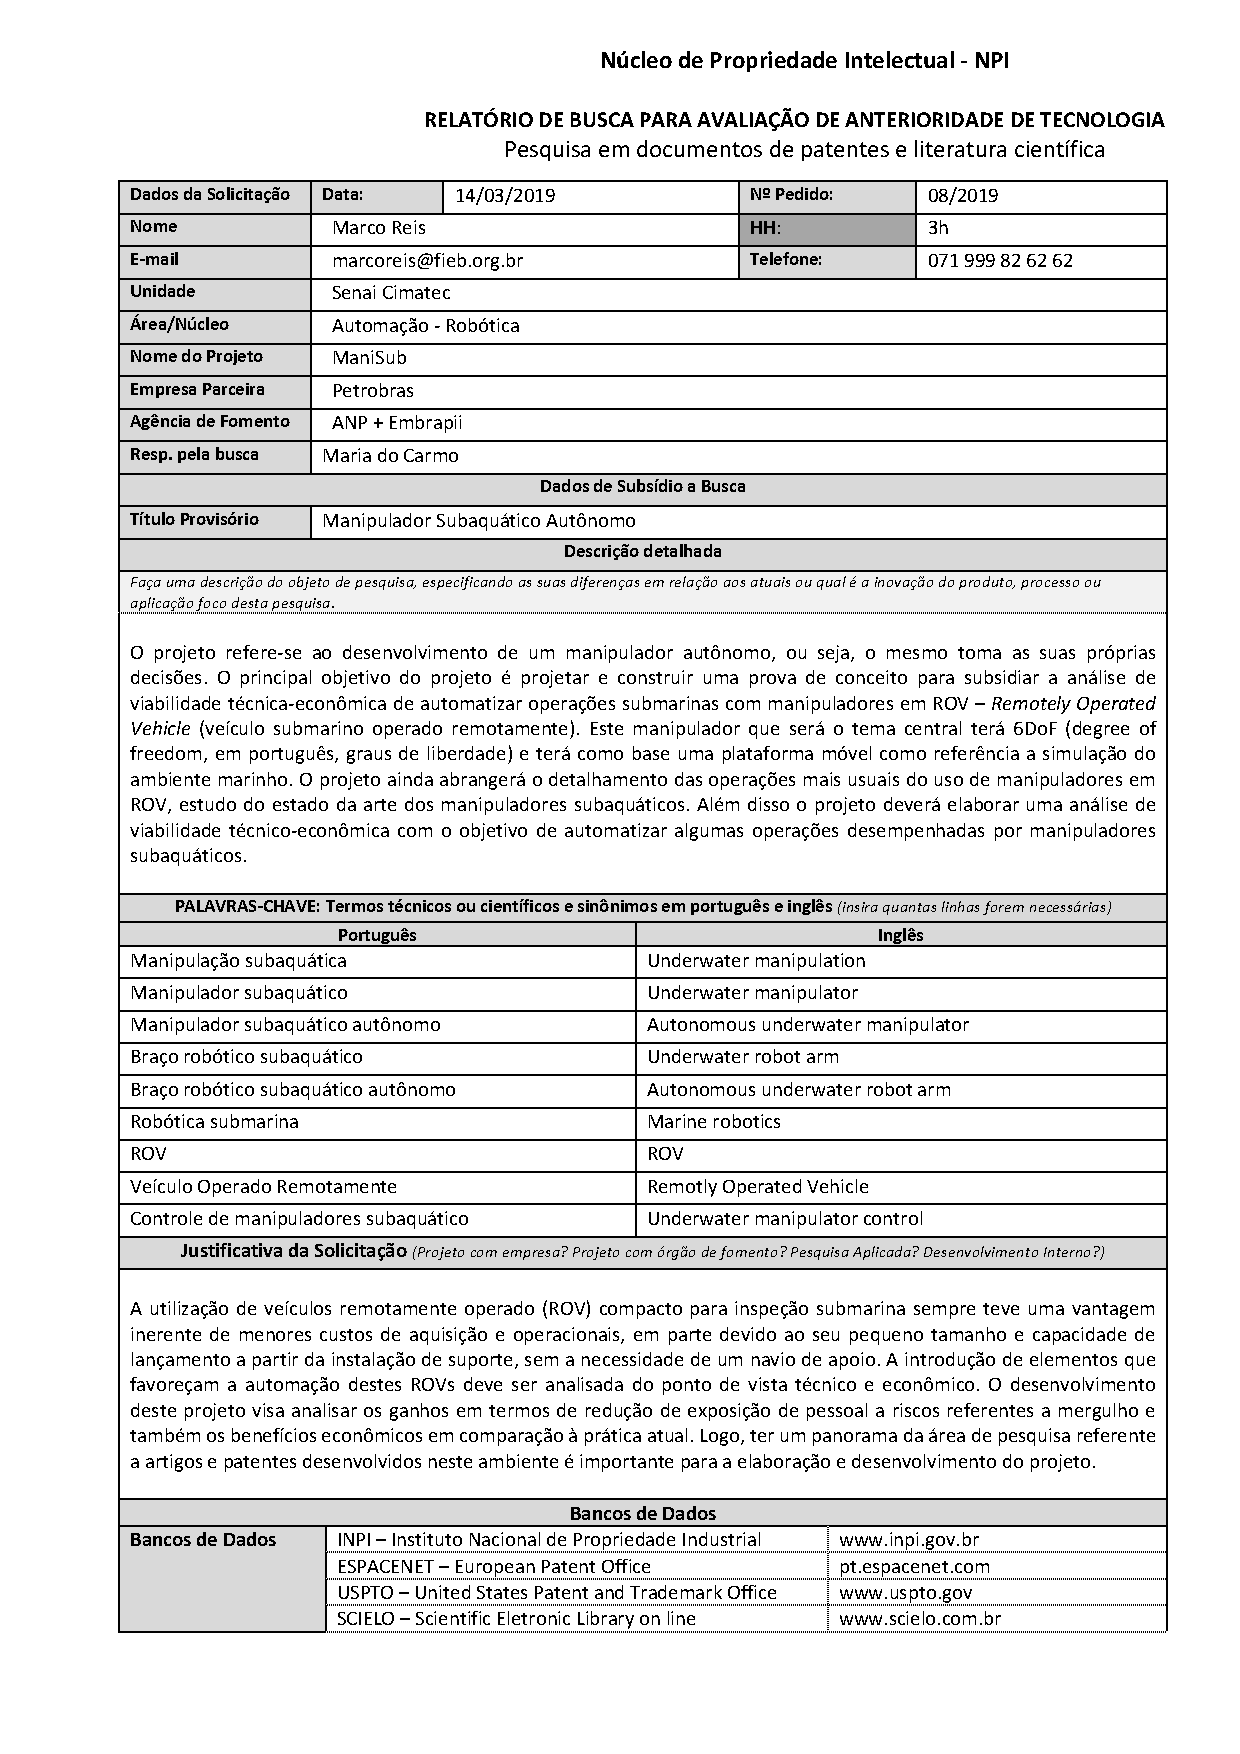
\includepdf[pages={{},-}]{annex/manisubanterioridade.pdf}
	% \lipsum[1] % Comentar e adicionar apêndice aqui
	% %
\end{document} 